\documentclass[a4paper]{article}

%% Language and font encodings
\usepackage[english]{babel}
\usepackage[utf8x]{inputenc}
\usepackage[T1]{fontenc}
\usepackage{cite}


%% Sets page size and margins
\usepackage[a4paper,top=3cm,bottom=2cm,left=3cm,right=3cm,marginparwidth=1.75cm]{geometry}

% header 2 char
\usepackage{indentfirst}
\setlength{\parindent}{2em}

%% Useful packages
\usepackage{amsmath}
\usepackage{graphicx}
\usepackage[colorinlistoftodos]{todonotes}
\usepackage[colorlinks=true, allcolors=blue]{hyperref}
\usepackage{cite}
\usepackage{amsfonts}

\title{\textbf{Neural Network Model Compression}}
\author{Zhao Xiaoyang, Lu Jikai, He Xiyuan}

\begin{document}
\maketitle

\section{Background}
\par Deep learning, one of the hottest areas in machine learning, has made lots of achievements on different applications. The success of deep learning is profited from not only the increasing amount of parameters, but also the large scale dataset contributed by both industrial and academical circles. To be specific, the large network model structure strengthen the ability of nonlinear curve fitting. Besides, Large scale data equipped the model with greater generalization ability.
\par However, when we apply deep network model to particular application, the performance will always be constrained by limited time or space. The cost not only relays on the number of parameters, but also the depth of the whole model. Especially for embedded, mobile and vision devices, it's very difficult to port the network model when the resources of cpu efficiency and memory are not as good as computer. Traditional deep network model's parameters represent the complexity and memory storage, but the local optimum for deploying parameters is not always the final requirements for application, which means some of these connections or weights may be redundant. Also, take residual model presented in \cite{residual} for example. Although it largely decreases the number of parameters compared to AlexNet, the deeper network generates lots of intermediary variables that are necessary in the backforward process. 
\par Given all above, compressing the neural network model is not simply decrease the number of parameters, accelerating the computing process through controlling the depth into a reasonable range is also necessary and worth exploring.

\section{Research Methods}
\subsection{Structure Changing}
\par The existing models of CNN lead research to focus on the improvement of lower latency and higher accuracy. However, with the increasing of model size and depth. Smaller CNN architectures definitely offer several advantages. Through adjusting the structure or way of computing convolution, the new model after changing may require less communication across servers during distributed training and less bandwidth to export a new model from cloud to certain platform. Besides, certain models are more feasible to deploy to mobile, embedded and memory-limited devices. The model represented in \cite{squeezenet} called SqueezeNet successfully achieve AlexNet-level accuracy on ImageNet with 50x fewer parameters and compress it 510x smaller than AlexNet. For the same purpose, MobileNets, introduced in \cite{mobilenets}, uses a set of two hyper-parameters to make itself a very small, low latency model which can be easily matched to the design requirements for mobile, embedded devices and especially vision application.
\subsubsection{SqueezeNet}
\par The design strategies mainly about three aspects.
\par The first strategy is to replace 3x3 kernel with 1x1 kernel. Developed from AlexNet to Deep Residual Learning presented in \cite{residual}, the convolution kernel mostly choose 3x3 because of it's efficient and simple to design. However, in order to reduce the number of parameters as well as keep the accuracy. The presented model partly uses 1x1 kernel and other 3x3 still.
\par The second strategy is decreasing the number of input channels to 3x3 filters. Through introducing squeeze layers, the model successfully solve the computing and storage burden caused by the whole quantity of parameters in a convolution layer. To be specific, a convolution layer contains totally (number of input channels)*(number of filters)*(3*3), just decrease the size of filter like strategy 1 is not always efficient. Decreasing the number of input channels is also necessary.
\par As for thee third strategy, we are supposed to downsample late in the network so that convolution layers have large activation maps. This idea actually based on the truth that larger activation maps can lead to higher classification accuracy. Thus in order to delay downsampling, the stride is set greater than 1 in some of the convolution or pooling layers. On the one hand, if early layers in the network have large strides, most will have small activation maps. On the other hand, most layers with a stride of 1 and those whose strides greater than 1 will concentrated toward the end of the network, thus leading to large activation maps.
\par The Figure \ref{squeeze} describes the building block called Fire Model, which is the key part of SqueezeNet and shows how to successfully employ the three strategies above to CNN architectures.
\par To build the whole SqueezeNet CNN architecture, we can begin with a standalone convolution layer, followed by 8 File modules, ending with a final conv layer. So actually, the third strategy can be applied by performing max-pooling with a stride of 2 after layers conv1, fire4, fire8, and conv10. Late placement of pooling successfully enlarge the activation maps, maximizing accuracy on a limited budget of parameters as a result.
\begin{figure}
\centering
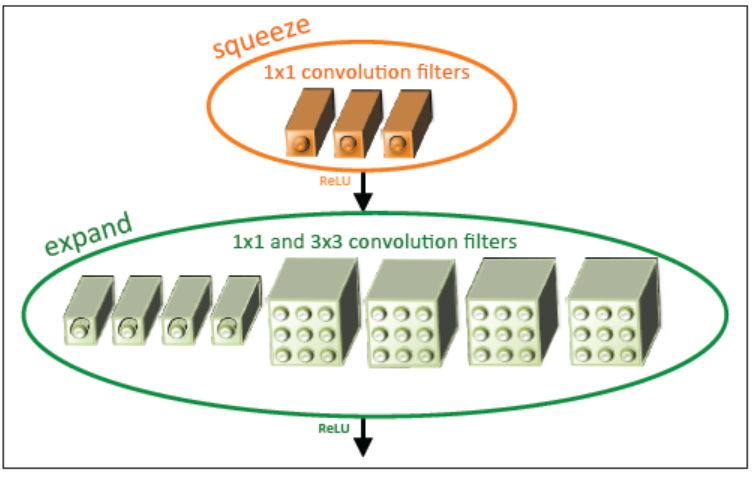
\includegraphics[width=0.6\textwidth]{squeeze1.png}
\caption{\label{squeeze}The Fire module is comprised of a squeeze layer and a following expand layer which has a set of 1x1 and 3x3 convolution filters. Here we use three hyper-parameters to control: $s_{1x1}$ determining the number of filters in squeeze layer, $e_{1x1}$ determining the number of 1x1 filters in expand layer, and $e_{3x3}$, which controls the 3x3 filters. Through adjusting the three hyper-parameters, the first two strategies can be implemented.}
\end{figure}

\subsubsection{MobileNets}
\par The model presented in \cite{mobilenets} called MobileNets introduces a great solution for mobile and embedded vision applications. The key idea of this model is to change the way of convolution computing though factorizing a standard convolution convolution into a depthwise convolution and a 1x1 pointwise convolution. The depthwise layer's filters only do convolution with each channel of input. The pointwise layer aims to combine the results from the earlier layers. This factorizing shown in Figure \ref{mobile} actually has the effect of drastically reducing computation and model size.
\par To further understand the strategy, we assume that the size of filter is $D_K$×$D_K$×N, where N represents the number of filters. If the input feature map in Figure \ref{mobile} (b) has number M, the output feature map is $D_F$×$D_F$×N, then the result computed from (b) will be $D_F$×$D_F$×M. The process (c) will finally get a feature map of $D_F$×$D_F$×N. Different from the standard process having a calculation amount $D_F$×$D_F$×$D_K$×$D_K$×$M$×$N$, the factorizing strategy decreases it into $D_F$×$D_F$×$D_K$×$D_K$×$M$+$D_F$×$D_F$×M×N. In another word, when the size of filer is 3x3, the time cost on doing convolution can be almost reduces to 9 times than before.
\par G.Howard also demonstrated how to build smaller and faster MobileNets using width multiplier and resolution multiplier by trading off a reasonable amount of accuracy to reduce size and latency. They model was compared to others on a wide variety of tasks and shows efficient performance, which also gives an direction to explore further. 
\begin{figure}
\centering
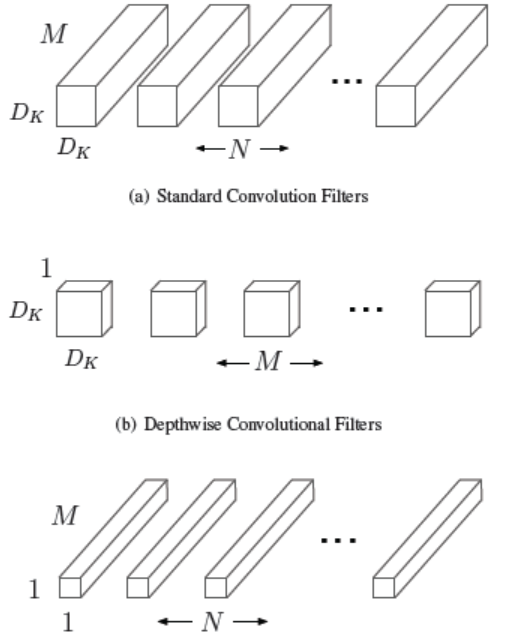
\includegraphics[width=0.5\textwidth]{mobile.png}
\caption{\label{mobile}Shows how a standard convolution layer factorized into depthwise and pointwise layer.}
\end{figure}

\subsection{Fine-Tuning on Trained Model}
\par Except the method of changing the structure and computing way of the whole network. It's also widely used to adopting strategies like pruning, low-rank decomposition and weights quantization to retrain the network and make it sparse after modification. Many great researchers like S.Han, Anwar, come up with many inspiring ideas to reduce the light connections in convolution and unnecessary memory for storage. Here we will summarize some classical theories can be applied to fine tuning on trained model.
\subsubsection{Pruning}
\par In the paper \cite{prunning} published by Stanford, the authors first come up with the ideas that through retrain the network by reducing unnecessary connections to decrease memory storage and cpu consuming. The key process contains three steps: first train the new work to learn which connections are important. Next, unimportant connections below the threshold are supposed to be pruned so that the network will become sparse. Finally, retrain the network to fine tune the weights of the remaining connections. However, following the three-step process, there are still some necessary measures to take. Choose the L2 regularization will result a better performance of pruning and retraining. During the training, the dropout ratio must be adjusted to account for the change in model capacity. And also, when retrain the pruned layers using a iterative way, the author keep the surviving parameters instead of re-initializing them.	
\par However, the traditional pruning\cite{prunning} strategy talked above has two major problems. The first is the possibility to prune important parameters accidentally because of the dynamic change of network connection importances. The other problem is the large consuming time in pruning process. Given this, a dynamic network surgery represented in \cite{dynamic} successfully compress the number of parameters in LeNet-5 and AlexNet without any accuracy loss. According to the author, the proposed method involves two key operations: pruning and splicing. In the pruning operation, unexpected accuracy losses are likely to happen, and the over pruning or incorrect pruning should be responsible for that. That's why the splicing process is necessarily needed in network surgery. Once the pruned connections are found to be important any time, the lost connection will recovery, adapting to the dynamic change of training network. 
\par Then in the paper \cite{structuredprunning} published in 2017, structured pruning was introduced at various granularities. Traditionally using randomly scattered sparsity in a network is very difficult to show computation advantages, thus the author uses a particular filtering approach to decide the importance of connections and paths, and provides many conditional operations and extra representation to denote the location of zero or non-zero parameters. In the experiments applying structured sparsity in deep convolution neural networks, the new method shows efficient performance on different tasks, different dataset like CIFAR-10 and MNIST.

\subsubsection{Low-Rank Decomposition}
\par Because networks are trained with a large number of output targets to achieve good performance, the majority of these paramaters are in the final weight layer. We propose a low-rank matrix factorization of the final weight layer. We apply this low-rank technique to our models, and we can see that a low-rank factorization reduces the number of parameters of the network by 30-50\%. This results in roughly an equivalent reduction in training time, without a significant loss in final recognition accuracy, compared to a full-rank representation.
\par Having a larger number of output targets contributes significantly to the large number of parameters in the system, as over 50\% of parameters in the network can be contained in the final layer. Furthermore, few output targets are actually active for a given input, and we hypothesize that the output targets that are active are probably correlated. The last layer is used to project the final hidden representation to these output targets. Because few output targets are active, we suspect that the false weight layer(i.e. matrix) has low rank. If the matrix is low-rank, we can use factorization to represent this matrix by two smaller matrices, thereby significantly reducing the number of parameters in the network before training. Another benefit of low-rank factorization for non-convex objective functions, is that it constrains the space of search directions that can be explored to maximize the objective function. This helps to make the optimization more efficient and reduce the number of training iteration.
\par The use of low-rank matrix factorization for improving optimization problems has been explored in a variety of contexts. Basically, there are three ways that we can take to do low-rank matrix decomposition.
\begin{enumerate}
\item Singular Value Decomposition\cite{singular}
\par Matrices are 2-tensors which can be linearly compressed using the Singular Value Decomposition. If W  \begin{math} \in \mathbb{R}^{m\times k} \end{math} is a really matrix, the SVD is defined as W = USV$^{T}$, where U \begin{math} \in \mathbb{R}^{m\times m} \end{math}, S \begin{math} \in \mathbb{R}^{m\times k} \end{math}, V \begin{math} \in \mathbb{R}^{k \times k} \end{math}. S is a diagonal matrix with the singular values on the diagonal, and U,V are orthogonal matrices. If the singular values of W decay rapidly, W can be well approximated by keeping only the t largest entries of S, resulting in the approximating \begin{math}\tilde{W} = \tilde{U} \tilde{S} \tilde{V} ^{T}\end{math}, where  \begin{math} \tilde{U} \in \mathbb{R}^{m\times t} \end{math}, \begin{math} \tilde{S} \in \mathbb{R}^{t \times t} \end{math},  \begin{math} \tilde{V} \in \mathbb{R}^{t \times k}\end{math}. Then, for I \begin{math} \in \mathbb{R}^{n\times m} \end{math}, the approximation error $\left \| I\tilde{W} -IW \right \|_{F}$ satisfies $\left \| I\tilde{W} -IW \right \|_{F} \leq s_{t+1} \left \| I \right \|_{F}$, and thus is controlled by the decay along the diagonal of S. Now the computation IW can be done in $O(nmt + nt^{2} + ntk)$, for sufficiently small t is significantly smaller than $O(nmk)$.


\item Tucker Decomposition\cite{tucker}
\par  Tucker decomposition is a higher order extension of the singular value decomposition (SVD) of matrix, in the perspective of computing the orthonormal spaces associated with the different modes of a tensor. It simultaneously analyzes mode-n matricizations of the original tensor, and merges them with the core tensor as illustrated in In our whole network compression scheme, we can apply Tucker-2 decomposition, which is also known as GLRAM\cite{glram}, from the second convolution layer to the first fully connected layers. 


\item Block Decomposition\cite{block}
\par To mitigate the inefficiency due to the single large circulant matrix used in, we can use block circulant matrices for weight representation. The benefits are twofold. First, it avoids the wasted storage/computation due to zero padding when the numbers of inputs and outputs are not equal. Second, it allows us to derive a fine-grained trade off between accuracy and compression/acceleration. Specifically, to achieve better compression ratio, larger block size should be used, however, it may lead to more accuracy degradation. The smaller block sizes provide better accuracy, but less compression. There is no compression if the block size is 1.
\end{enumerate}


\subsubsection{Weights Quantization}

\par As we know, the key factor for the progress of Deep Neural Network is the advent of GPU. Therefore, the research for deep-learning on some low-power devices is extremely important. Previous work \cite{binary} focus on the compression for weights. It has shown that by constrain the weights in the forward and backward propagation, we can get the state-of-art result with the BinaryConnect method.
\par There are two ways to transform the real-weight value to the two possible values. The first is a deterministic method and the second is a stochastic method. In the stochastic method, we can use the \emph{hard sigmoid} function because it requires less calculation than soft version. Then we should consider the training process. We can simply divide the process into three steps. First, from the bottom of the network, we calculate the unit activation layer by layer. Second, we calculate the gradient from the top to the bottom layer by layer, namely the back propagation. At last, we update the parameters. The most important thing is that we should only binarize the weights in the forward and backward propagations but not in the parameter update process. To make SGD work out well, we should keep the precision of weights.


\par Besides the BinaryConnect method, weights quantization and weight sharing can further compress the network by reducing the storage for all the weights. In the traditional network, weights are usually stored in the format of float. Therefore, we have to store all the weights for a small network. However, a great number of weights are similar and they can be represented by a single centroid. It is obvious that by clustering these weights, the space for network will be largely saved. Experiment \cite{deepcompress} has shown that after the weight quantization and sharing, the accuracy of network does not drop. 
\par Assume that  the number of weights is \emph{n}, and each connection is represented by \emph{b} bits, then the previous space for the network is \emph{nb} bits. Using the method above, we only need \emph{$n\log_2k+kb$}  to store the weight.
\par We can use k-means to solve the clustering problem. There are three ways to initialize the centroid, namely the forgy method(random), the density-based method and the linear method. It shows that the training result of the weights usually has two peaks \cite{deepcompress}. The forgy and density-based method cannot cover the large weights well. Therefore, linear initialization is a better solution. 
\par To further save the storage, we can use the Huffman Coding to store the index of these weights. Huffman Coding uses variable-length codewords to encode the index. We have mentioned above that there exist two peaks in the weight distribution graph, so we can use a shorter codeword to store the weight near the peaks. 



\par On the base of the previous work, researchers come up with another method called Trained Ternary Quantization \cite{ternary}. Instead of using the \{-1, 0, +1\} values, the negative and positive weights can be learned in the training process. The first step is normalize the precise weights to the range of [-1, +1] by dividing all the weights by the maximum weight. Then we choose a threshold factor to divide the weights into three labels. At last, we will back-propagate two gradient, namely one to the full-resolution weights and another to the scaling coefficients. Then the positive and negative weights will be trained together with other parameters. Experiment shows that the ternary model reaches or even surpasses the performance of the full precision model. 

\section{Experiment Evaluation}
\par Recently, research papers about deep compressing mostly evaluated their performances on large models like AlexNet and Vgg. In our own implement to compress existing models, we choose Lenet-5(see Figure \ref{lenet}) to do test and use Mnist dataset to train the compressed model. To achieve that, we basically follow the idea come up with S.Han\cite{deepcompress} to do pruning and quantization on fully-connection layer and convolution layer. However, different from what he did on AlextNet, we aim to prevent the decreasing of accuracy through modifying the source code of caffe.
\begin{figure}
\centering
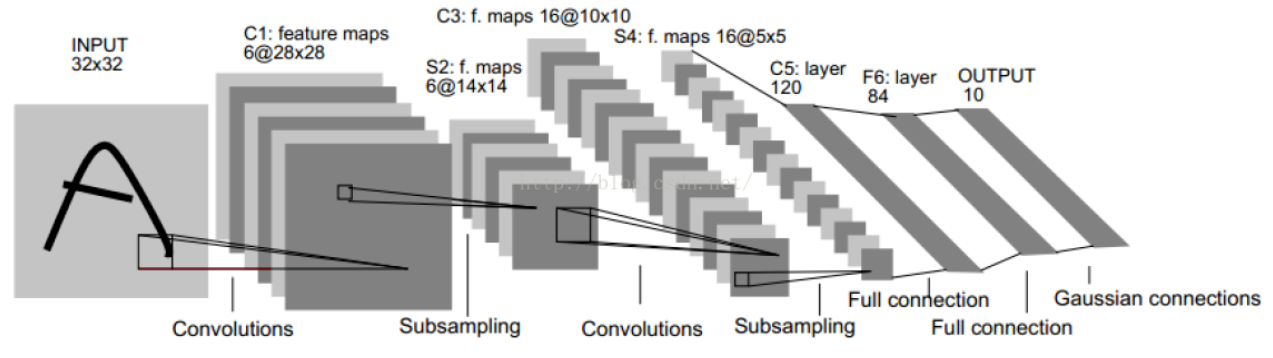
\includegraphics[width=0.9\textwidth]{lenet.png}
\caption{\label{lenet}The traditional process of a lenet model applying on handwriting recognition problem.}
\end{figure}

\par To be specific, from the view of network model, we add two own defined layers called \textit{CmpConvolution} and \textit{CmpInnerProduct}. In the two layers, we introduce three important parameters:
\begin{itemize}
\item sparse\_ratio
\item class\_num
\item quantization\_term
\end{itemize}
\par They respectively represents pruning rate, number of cluster centers in k-means and whether choose to do quantization. According to the idea in paper, we firstly set the sparse\_ratio of each layer to be 0.33(cov1), 0.8(cov2), 0.9(fc1), 0.8(fc2) before training.
\par From the view of caffe source, that's where we take specific pruning and quantization strategies. Take the convolution layer for example, we define a mask to shield the pruned weight, an indice to store the reference number, and a centroid structure to keep the cluster center. They are added into the layer class as member variables. Besides, we also modified the forwarding and backwarding function. In the forward process, we use cluster center to represent the weights. And in the backward, we need to divide the situation into two parts to take different measures. First, for those whose mask variable is 0, regard it as pruned and ignore the updating process. Second, summary every cluster's gradient difference and back propagate the result.
\par In practice, the layers are much more sensitive to weight pruning than weight quantization. Therefore, we first set the sparse ratio (the ratio of pruned weights) layer-wisely and do each fine tuning iteration. After all layer are properly pruned, weight quantization can then be done on all layers simultaneously. Finally, in order to decrease the size of model, we only store the non-zero weight, index and the cluster center using float32 data type.

%result
\par The model after fine tuning shows a great decrease in the number of parameters. The original model takes about 1720KB memory for parameters storage, while the compressed model only takes about 44KB. The compress rate is nearly 40×. However, the accuracy doesn't decrease. It reaches about 99.06\% when tested on MNIST dataset to identify handwriting digits.
\par There are still some limitations in our experiments. On the one hand, at the bottom of caffe, the \textit{.cu} files still call the interface of \textit{cpu\_data}, which may cause an extra time consuming while exchanging data with gpu. On the other hand, how to automatically select a threshold still need to be solved. In a word, if we want to port CNN model into embedded devices, the model structure, model quantization and \textit{NEON} instruction accelerating also need to be considered.

\section{Improvements}
\par According to the related work and the experiments results we got, we can see that some problems still remain to be explored further. \par First, how to precisely measure the influence on training results caused by weights parameters is of vital importance but also difficult to find a efficient solution. The way we use now to measure the kernel and kernel weight is still very simple. Although the paper \cite{design} gives an analysize about that, it has a great amount of calculation and is hard to be applied. 
\par Second, a large scale of network tends to be trained on a huge dataset. For example, the model trained through ImageNet has the ability to classify one thousand kinds of objects. However, in some particular applications, we simply need to identify certain subjects through smaller sub-model. Thus, how to compress the model from the perspective of application is still an opening question.
\par Third, there is a lack of compress evaluation system. Related researches focus on the comparison of running time and number of parameters, which is not generalized enough. Future researches can be done to present a  evaluation criterion. On the one hand, consider the performances on different applications and find the balance between them. On the other hand, evaluating the compressed model from the structure of model itself is also necessary.

\bibliographystyle{unsrt}
\bibliography{sample.bib}
\end{document}